\title{Asymmetric hyperbolic L-spaces, \\ 
\mbox{}\hspace{1.5cm} Heegaard genus, and Dehn filling}

\author{Nathan M. Dunfield}
\givenname{Nathan}
\surname{Dunfield}
\address{ Dept.~of Math., MC-382 \\
          University of Illinois \\
          1409 W. Green St. \\
          Urbana, IL 61801 \\ 
          USA
}
\email{nathan@dunfield.info}
\urladdr{http://dunfield.info}

\author{Neil R. Hoffman}
\givenname{Neil}
\surname{Hoffman}
\address{Dept.~of Math. and Stat. \\
University of Melbourne\\
Parkville, VIC 3010 \\
Australia}
\email{nhoffman@ms.unimelb.edu.au}
\urladdr{http://ms.unimelb.edu.au/~nhoffman/}

\author{Joan E. Licata}
\givenname{Joan}
\surname{Licata}
\address{Mathematical Sciences Institute\\
John Dedman Bldg 27\\
The Australian National University 0200\\
 Australia}
\email{joan.licata@anu.edu.au}
\urladdr{http://maths-people.anu.edu.au/~licataj/}

\arxivreference{}
\arxivpassword{}

% AMS style garbage
%\subjclass[2000]{57} % Really these are 2010 MSC numbers
%\keywords{}
% GT style garbage
%\subject{primary}{msc2010}{57}
%\subject{secondary}{msc2010}{57}
%\keyword{}


\newcommand{\centercolhead}[1]{\multicolumn{1}{c}{#1}}
\newcommand{\Na}{N_\alpha}
\newcommand{\Nb}{N_\beta}
\newcommand{\HoneZ}[1]{H_1(#1; \Z)}
\newcommand{\HoneZbdryN}{\HoneZ{\partial N}}
\newcommand{\ZHS}{$\Z \mathrm{HS}$}
\newcommand{\tilt}[1]{\mathrm{Tilt}\!\left(#1\right)}
\newcommand{\interval}[1]{[#1]}
\newcommand{\inta}{\interval{a}}
\newcommand{\intb}{\interval{b}}
\newcommand{\intC}{\interval{C}}
\newcommand{\intCone}{\interval{C_1}}
\newcommand{\intCzero}{\interval{C_0}}
\newcommand{\intCp}{\interval{C^+_1}}
\newcommand{\intCm}{\interval{C^-_1}}
\newcommand{\inputfig}[1]{\input{figs_and_tables/#1}}

%  document starts
\begin{document}

\begin{abstract} 
  An $L$-space is a rational homology 3-sphere with minimal Heegaard
  Floer homology.  We give the first examples of hyperbolic $L$-spaces
  with no symmetries.  In particular, unlike all previously known
  $L$-spaces, these manifolds are not double branched covers of links
  in $S^3$.  We prove the existence of infinitely many such examples
  (in several distinct families) using a mix of hyperbolic geometry,
  Floer theory, and verified computer calculations.  Of independent
  interest is our technique for using interval arithmetic to certify
  symmetry groups and non-existence of isometries of cusped hyperbolic
  3-manifolds. In the process, we give examples of 1-cusped hyperbolic
  3-manifolds of Heegaard genus 3 with two distinct lens space
  fillings.  These are the first examples where multiple Dehn fillings
  drop the Heegaard genus by more than one, which answers a question
  of Gordon.
\end{abstract}
\maketitle


 \section{Introduction}
\subsection{Asymmetric \emph{L}-spaces}
For a rational homology \3-sphere $M$, the rank of its Heegaard Floer
homology $\HFhat(M)$ is always bounded below by the order of
$\HoneZ{M}$, and $M$ is called an \textit{$L$-space} when this bound is an
equality.  Lens spaces and other spherical manifolds are all
$L$-spaces, but these are by no means the only examples.  In fact, recent
work of Boyer, Gordon, and Watson \cite{BoyerGordonWatson2013} shows
that each of the eight \3-dimensional geometries has an
$L$-space. Their work is part of broader efforts to characterize
$L$-spaces via properties not obviously connected to Heegaard
Floer theory; specifically, they conjecture that a rational homology
sphere is an $L$-space if and only if its fundamental group is not
left-orderable. Although the conjecture has been resolved for seven of
the geometries, it remains open for the important case of hyperbolic
geometry as well as for most manifolds with non-trivial JSJ
decompositions.  Previous constructions of hyperbolic $L$-spaces
produce them via surgery on strongly invertible manifolds, leading to
examples which are double branched covers over links in $S^3$.  One of
our main results  shows that these are constructions of convenience
rather than necessity.  Recall that a hyperbolic 3-manifold is
\emph{asymmetric} if its only self-isometry is the identity map; by a
deep theorem of Gabai, this is equivalent to every self\hyp
diffeomorphism being isotopic to the identity \cite{Gabai2001}.  We
will show the following:
 \begin{theorem}\label{thm:main} 
   There exist infinitely many asymmetric hyperbolic $L$-spaces.  In
   particular, there are hyperbolic $L$-spaces which are neither
   regular covers nor regular branched covers of another \3-manifold.
\end{theorem}
\noindent 
Among $L$-spaces which are \emph{not} double branched covers over
links in $S^3$, hyperbolic examples such as those of
Theorem~\ref{thm:main} are the simplest possible in the sense that any
such $L$-space must have a hyperbolic piece in its prime/JSJ
decomposition.  This is because any graph manifold which is a rational
homology sphere, much less an $L$-space, is a double branched cover
over a link in $S^3$. %, see Proposition~\ref{prop:branch}.
This was proved by Montesinos in
\cite[$\S$7.2]{montesinos1973variedades}; the theorem stated there is
paraphrased %(he refers to graph manifolds as ``Waldhausen manifolds'')
in the translation below: 
\begin{theorem}[{\cite[$\S$7.2]{montesinos1973variedades}}]
Let $M$ be a graph manifold whose diagram is a tree with each vertex  corresponding to a Seifert fibered space over
a (punctured) $S^2$ or (punctured) $\RP^2$. 
Then $M$ is a double branched cover of a link $L$ in $S^3.$ 
\end{theorem}
\noindent
Note the rational homology sphere assumption implies that the diagram
of the graph manifold is a tree. Also, the cases that arise if the tree is a just single vertex are covered in \cite[$\S$2-3]{montesinos1973variedades}.

\begin{figure}
  \begin{center}
   \inputfig{L12n1314}
  \end{center}
  \caption{The link used in Theorem~\ref{thm:link} is $L12n1314$ in
    the Hoste-Thistlewaite census. Our framing conventions for Dehn
    filling are
    \protect\raisebox{-0.1cm}{\protect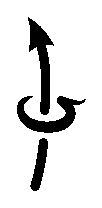
\includegraphics[angle=90,
      scale=0.35]{figs_and_tables/orientation}} and are consistent
    with SnapPy \cite{SnapPy}.  Note there is an
    orientation-preserving homeomorphism of $S^3$ which interchanges
    the two components.  }\label{fig:link}
\end{figure}


We prove Theorem~\ref{thm:main} via a combination of hyperbolic
geometry, Heegaard Floer theory, and verified computer calculations.
The proof of Theorem~\ref{thm:main} has two parts, the second of which
is computer-aided.  The first result shows that we need only construct
1-cusped manifolds with certain properties, and the second establishes
the existence of such manifolds.  Here, the \emph{order} of a lens
space is the order of its fundamental group/first homology.

\begin{restatable*}{theorem}{theoremtheory}\label{thm:theory}
  Suppose $M$ is a 1-cusped hyperbolic \3-manifold.  If $M$ is
  asymmetric and has two lens space Dehn fillings of coprime order,
  then there are infinitely many Dehn fillings of $M$ which are
  asymmetric hyperbolic $L$-spaces. Moreover, $M$ is the complement of
  a knot in an integral homology \3-sphere and fibers over the circle
  with fiber a once-punctured surface.
\end{restatable*}

\begin{restatable*}{theorem}{theoremlink}\label{thm:link}
  There exist infinitely many 1-cusped hyperbolic \3-manifolds which
  are asymmetric and have two lens space fillings of coprime order.
  Specifically, if $N$ is the exterior of the link in
  Figure~\ref{fig:link}, then for all large $k \in \Z$, the $(6k\pm1,
  k)$ Dehn filling on either component of $N$ yields such a manifold.
\end{restatable*}
\noindent
In addition to Theorem~\ref{thm:link}, Theorem~\ref{thm:comp} 
offers a finite number of explicit examples for which the proof is
slightly easier.  A Heegaard diagram of the simplest of these examples
is given in Figure~\ref{fig:v3372}.  

\subsection{Heegaard genus,  Dehn filling, and the Berge conjecture} 
Our second main result answers a question of Gordon
\cite{GordonAIM} regarding the existence of manifolds where multiple
fillings drop the Heegaard genus by more than one:
\begin{corollary}\label{cor:genusdrop}
  There exist infinitely many 1-cusped hyperbolic \3-manifolds of
  Heegaard genus three which admit two distinct lens space fillings.
\end{corollary}
\noindent
This corollary follows immediately from Theorem~\ref{thm:link}, as
manifolds with genus two Heegaard splittings always have symmetries; 
 the examples of Theorem~\ref{thm:link} must have Heegaard
genus exactly three since the link in Figure~\ref{fig:link} is
\3-bridge. 

The interest in $L$-spaces stems in part from open questions about
lens space surgery, with the Berge Conjecture as the chief example.
Another interesting feature of Corollary~\ref{cor:genusdrop} is that
it provides counterexamples to the following generalization of the
Berge Conjecture, since the exterior of any $(1,1)$--knot has Heegaard
genus two:

\begin{conjecture}[{\cite[Conjecture 9]{BakerDoleshalHoffman}}] 
  If knots $K_1 \subset L(p_1, q_1)$ and $K_2 \subset L(p_2,q_2)$ are
  longitudinal surgery duals, then up to reindexing, $K_2$ is a
  $(1,1)$--knot and $p_2 \geq p_1$.
\end{conjecture}
\noindent
We note that these examples do
not contradict the Berge Conjecture itself because they are not
knot complements in $S^3$; see the proof of Theorem~\ref{thm:link} for details.

\section{Asymmetric L-spaces from cusped manifolds}

This section is devoted to the proof of the following result:
\theoremtheory
\noindent
This theorem follows immediately from the next two lemmas, where in
the second one we set $N \setminus \partial N \cong M$. 

\begin{lemma}\label{lem:hyperdehn}
  Suppose $M$ is an asymmetric 1-cusped hyperbolic \3-manifold.  Then
  all but finitely many Dehn fillings of $M$ are hyperbolic and asymmetric.
\end{lemma}

\begin{lemma}\label{lem:floer}
  Suppose $N$ is a compact \3-manifold with $\partial N$ a torus.  If
  $N$ has two lens space Dehn fillings of 
  coprime order, then $N$ has infinitely many Dehn fillings which are
  $L$-spaces.  Moreover, $N$ is the exterior of a knot in an integral
  homology sphere and fibers over the circle with fiber a surface with
  one boundary component.
\end{lemma}

The proofs of these two lemmas are completely independent and will be
familiar to experts in the areas of \3-dimensional hyperbolic geometry and
Heegaard Floer theory, respectively. 


\section{Asymmetric manifolds with lens space fillings}\label{sect:comp}

Before proving Theorem~\ref{thm:link}, we warm up with the following
easier and more concrete result, which, when combined with
Theorem~\ref{thm:theory}, also suffices to prove
Theorem~\ref{thm:main}.
\begin{restatable}{theorem}{theoremcomp}\label{thm:comp}
  Table~\ref{table:examples} lists 22 distinct 1-cusped hyperbolic
  \3-manifolds which are asymmetric and have two lens space fillings
  of coprime order.
\end{restatable}
\noindent
We provide a rigorous computer-assisted proof of
Theorem~\ref{thm:comp} using SnapPy \cite{SnapPy}, the verification scheme
of \cite{hikmot2013verified}.  These examples were found in the census
of 1-cusped hyperbolic \3-manifolds with at most 9 tetrahedra
\cite{Burton2014, CallahanHildebrandWeeks1999} by a 
brute-force search through these 59{,}107 manifolds.
\begin{table}
\small
  \begin{center}
    \inputfig{table.tex}
  \end{center}
  \caption{The 22 manifolds of Theorem~\ref{thm:comp}.  Here, ``\#tets'' refers to the
    canonical triangulation supplied in \cite{ancillary} and $g$ is the genus of the fibration
    of $M$ over the circle (whose existence follows from
    Theorem~\ref{thm:theory}) computed via the Alexander
    polynomial.  The lens spaces were identified using Regina
    \cite{Regina}.  The manifolds marked with a $*$ also appear in
    Theorem~\ref{thm:link}.    The
    data is all rigorous with the exception of the volume and systole
    columns, which were approximated numerically, as the methods of
    \cite{hikmot2013verified} have not yet been extended to those
    quantities.  Note that
    none of these manifolds are knot complements in $S^3$, since the
    pair of lens space surgeries have fundamental groups whose orders
    differ by more than one.}\label{table:examples}
\end{table} 
\begin{figure}
  \vspace{-0.7cm}
  \begin{center}
    \inputfig{heegaard}
    %M = snappy.Manifold('v3372')
    %sage: G = M.fundamental_group()
    %sage: G
   % Generators:
    %  a,b,c
    %Relators:
     % aBAAccbc
     % abAccbaabcb
    %sage: G.peripheral_curves()
    %[('CCaab', 'cbaa')]
  \end{center}
  \vspace{-1.75cm}
  \caption{A Heegaard diagram for the first manifold $v3372$ in
    Table~\ref{table:examples}, corresponding to 
    $\big\langle a,b,c \  \big| \ R_1 := ab^{-1}a^{-2}c^2bc = 1, \  R_2 := aba^{-1}c^2ba^2bcb = 1 \big\rangle$. 
    Also shown are
    the slopes $\alpha = c^{-2}a^2b$ and $\beta = cba^2$
    which give lens spaces $L(7,1)$ and $L(19,7)$, 
    oriented so any positive combination of them gives an
    $L$-space.
  }\label{fig:v3372}
\end{figure}


We next extend the phenomena exhibited in
Theorem~\ref{thm:comp} to an infinite family of examples; note  that our conventions for Dehn
filling are specified in Figure~\ref{fig:link}.

\theoremlink

\begin{figure}
  \begin{cxyoverpic}{(169,206)}{scale=0.80}{figs_and_tables/2fusion-link}
    ,(1,150)*+!R{C_2}
    ,(5,111)*++!R{C_1}
    ,(15,36)*++!R{C_0}
  \end{cxyoverpic}
  \caption{The link $L$.}
  \label{fig-2fusion-link}
\end{figure}



{\RaggedRight \bibliographystyle{nmd/math}
  \small
  \bibliography{article} }
\end{document}
